\chapter{REPORT} \label{ch:procedure}
\section{Functional Requirements:}

\subsection{Vendor Subscription, Registration and Login}
This system handles the complete onboarding process for vendors joining the platform. It includes a registration form where vendors provide business details and upload legal documents (Trade License, E-TIN). Upon successful registration, vendors select and pay for a subscription plan (Basic or Professional) through integrated payment gateways. The login system implements Two-Factor Authentication (2FA) using OTP sent to email or phone, ensuring secure access to vendor dashboards. Each vendor receives a unique tenant ID and subdomain for their isolated store.



\subsection{Discount, Offers and Theme Customization}
This system enables vendors to create promotional campaigns and personalize their storefront appearance. Vendors can create percentage-based discounts (e.g., 20\% off), fixed-amount discounts, and "Buy X Get Y" offers (e.g., Buy 2 Get 1 Free). They can set start/end dates and usage limits (e.g., first 50 customers). The theme customization feature allows vendors to upload logos, select brand colors, choose layout templates, and customize navigation menus—all with live preview before publishing changes to their live store.


\subsection{Payment gateway system}
This system processes customer payments for orders placed on vendor stores. It integrates with multiple payment gateways including bKash, Nagad, Visa, and MasterCard, as well as supporting Cash on Delivery (COD). Customers select their preferred method during checkout. For online payments, the system redirects to the gateway and waits for confirmation before finalizing the order. Payment statuses (Paid, Failed, Pending) are tracked and updated accordingly. The system also generates transaction logs for audit purposes.

\subsection{Inventory Management and Analytics}
This module allows vendors to manage their product stock efficiently. Vendors can add new products, update stock quantities, set reorder levels, and receive low stock alerts. The system tracks stock movements (sales, restocks, adjustments) and maintains accurate inventory counts. Vendors can view inventory valuation, monitor stock turnover rates, and generate inventory reports. The module ensures that each vendor's inventory data remains isolated within their own tenant database, preventing data leakage between competing businesses.

\subsection{Customer Feedback, Product ratings and reviews}
This module enables customers to share their product experiences and helps vendors build trust. After purchasing a product, verified customers can submit star ratings (1 to 5 stars) and written reviews, optionally with photos. Reviews are displayed on product pages along with average ratings. Vendors can view pending reviews, approve or reject inappropriate content, and respond to customer feedback. The system tracks helpful votes and provides review analytics (average rating, distribution, response rates) to help vendors improve their products and customer satisfaction.


\section{Non-Functional Requirements}

\subsection{Data Isolation \& Security (Confidentiality)}
Metric: Since we are using a multi-tenant "Database-per-Tenant" design, the system must ensure 100\% data isolation. No cross-tenant query should be possible.

\subsection{Scalability \& Performance}
Metric: The Analytical Board and Inventory Management systems must handle concurrent updates. The system should maintain a response time of < 2 seconds for dashboard loading, even when 500+ vendors are accessing their respective databases simultaneously.

\subsection{High Availability \& Reliability}
Metric: Given that this is a subscription-based "Independent Storefront" model, the system must guarantee 99.9\% uptime. If the Payment Gateway or the Database-per-Tenant service fails, it must have a failover mechanism so vendors don't lose sales during peak promotional hours.

\section{User Stories}

\subsection{User Story for Multi-Tenant Architecture and Secure Vendor Management}

As an \textbf{entrepreneur (vendor)}, I want to register my business and subscribe to the platform to create my own digital storefront, so that I can manage products, customers, and orders online. The system should ensure that each vendor’s data is stored in an isolated database, preventing access by other vendors. Additionally, secure authentication and verification mechanisms must be implemented to protect vendor accounts and business information.

\subsection{User Story for Comprehensive Store Operations and Inventory Management}

As a \textbf{vendor}, I want to manage my store operations through a centralized dashboard, so that I can easily control inventory, create promotional offers, track sales analytics, and customize the visual appearance of my storefront. The system should provide real-time inventory updates and operational tools, enabling vendors to efficiently manage their online business from a single platform.

\subsection{User Story for Integrated Checkout, Payment, and Order Fulfillment}

As a \textbf{customer}, I want to complete purchases using multiple payment options such as online payment or Cash on Delivery, so that I can choose the most convenient payment method. The system should also integrate with third-party delivery services to provide real-time order tracking, allowing both customers and vendors to monitor the shipment status easily.

\section{Use Case Diagram}

\begin{figure}[H]
    \centering
    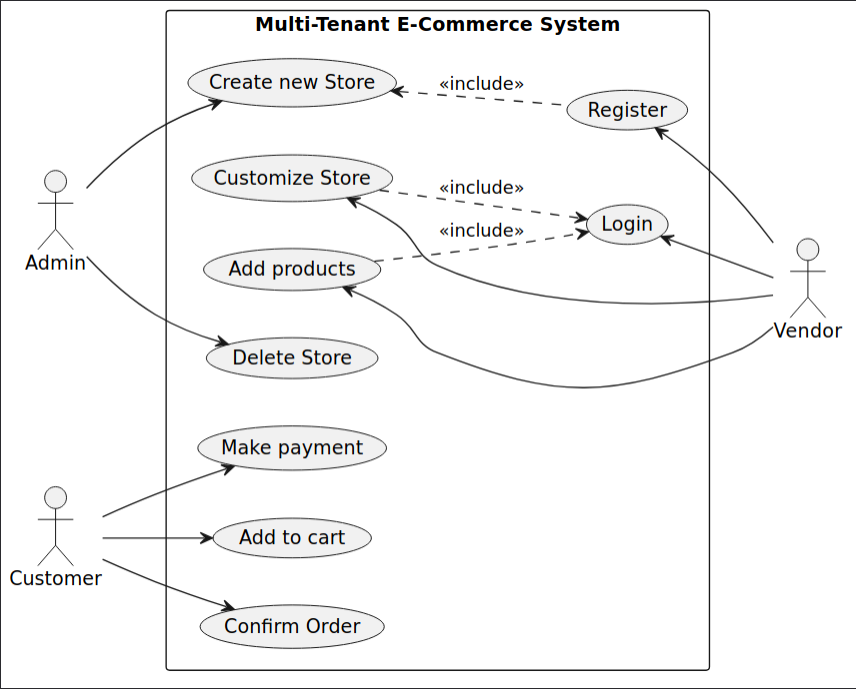
\includegraphics[width=1\linewidth]{figures/UseCaseDiagaram.png}
    \caption{Use Case Diagram for Multi-Tenants E-Commerce System}
    \label{fig:placeholder}
\end{figure}

\section{Use Case Specifications}

\subsection{Vendor Registration and Store Creation}

\textbf{Use Case Name:} Vendor Registration and Store Creation

\textbf{Actor}: Vendor (Entrepreneur)

\textbf{Description:} Allows entrepreneurs to register their business, subscribe
to the platform, and create an independent digital storefront with
isolated data storage.

\textbf{Preconditions:} Vendor has valid business and contact information. -
Vendor has internet access.

\begin{comment}
\textbf{Main Flow:} 1. Vendor enters business registration details. 2. Vendor
selects a subscription plan. 3. Vendor completes account verification
(email/OTP). 4. Platform creates a digital storefront with isolated
database.
\end{comment}

\textbf{Postconditions:} Vendor account is created and verified. - Independent
storefront is activated with isolated data storage.

\subsection{Store Operations and Inventory Management}

\textbf{Use Case Name:} Store Operations and Inventory Management

\textbf{Actor:} Vendor

\textbf{Description:} Allows vendors to manage store operations through a
centralized dashboard including product management, inventory updates,
promotions, analytics, and storefront customization.

\textbf{Preconditions:} Vendor account exists. - Vendor is logged into the
platform.

\begin{comment}    
\textbf{Main Flow:} 1. Vendor accesses the dashboard. 2. Vendor adds or updates
product listings and inventory. 3. Vendor creates promotional offers or
discounts. 4. Vendor views sales analytics and customizes storefront
appearance.
\end{comment}

\textbf{Postconditions:} Store products, inventory, and promotions are
updated. - Storefront configuration changes are applied.

\subsection{Checkout, Payment, and Order Tracking}

\textbf{Use Case Name:} Product Purchase and Order Fulfillment

\textbf{Actor:} Customer

\textbf{Description:} Allows customers to purchase products using multiple payment
methods and track order delivery through integrated logistics services.

\textbf{Preconditions:} Customer selects products. - Products are available in
stock.

\begin{comment} 
\textbf{Main Flow:} 1. Customer adds products to the shopping cart. 2. Customer
proceeds to checkout and enters delivery details. 3. Customer selects
payment method (online payment or Cash on Delivery). 4. Order is
confirmed and sent for delivery.
\end{comment}

\textbf{Postconditions:} Order is recorded in the system. - Customer and vendor
can track the delivery status.
\section{UML Class Diagram}

\begin{figure}[H]
    \centering
    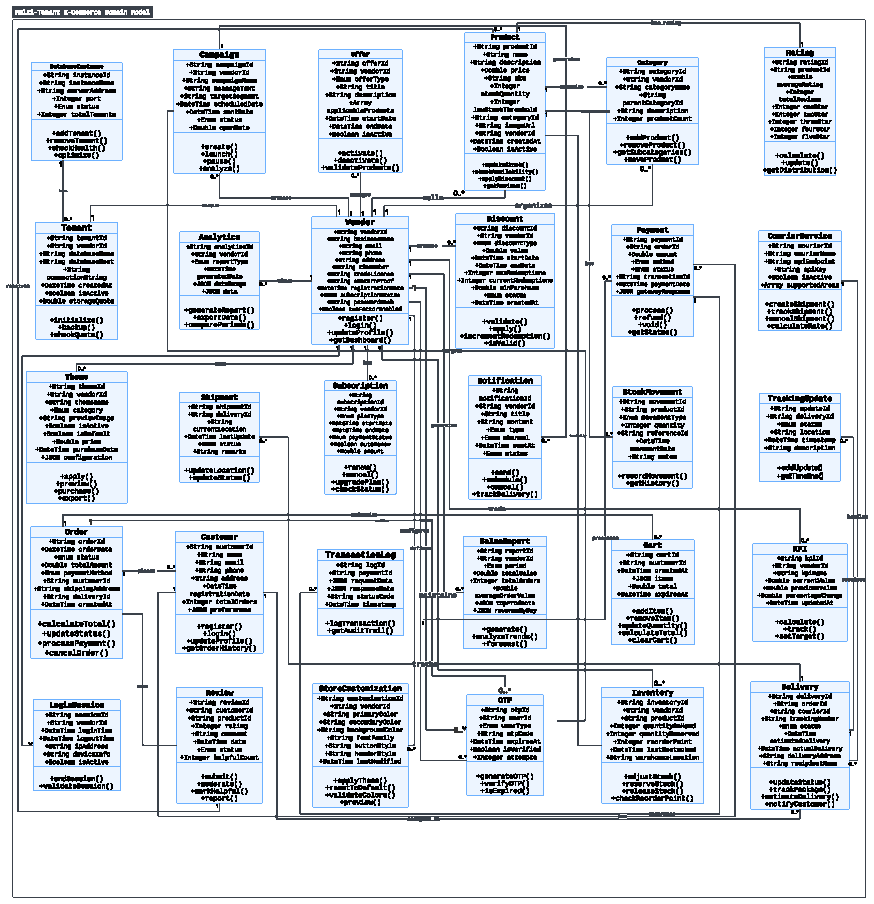
\includegraphics[width=1\linewidth]{figures/UML Class Diagram.pdf}
    \caption{UML Class Diagram for Multi-Tenants E-Commerce System}
    \label{fig:placeholder}
\end{figure}



\section{Sequence Diagram}

\subsection{Registration & Login Process Sequence}

\begin{figure}[H]
    \centering
    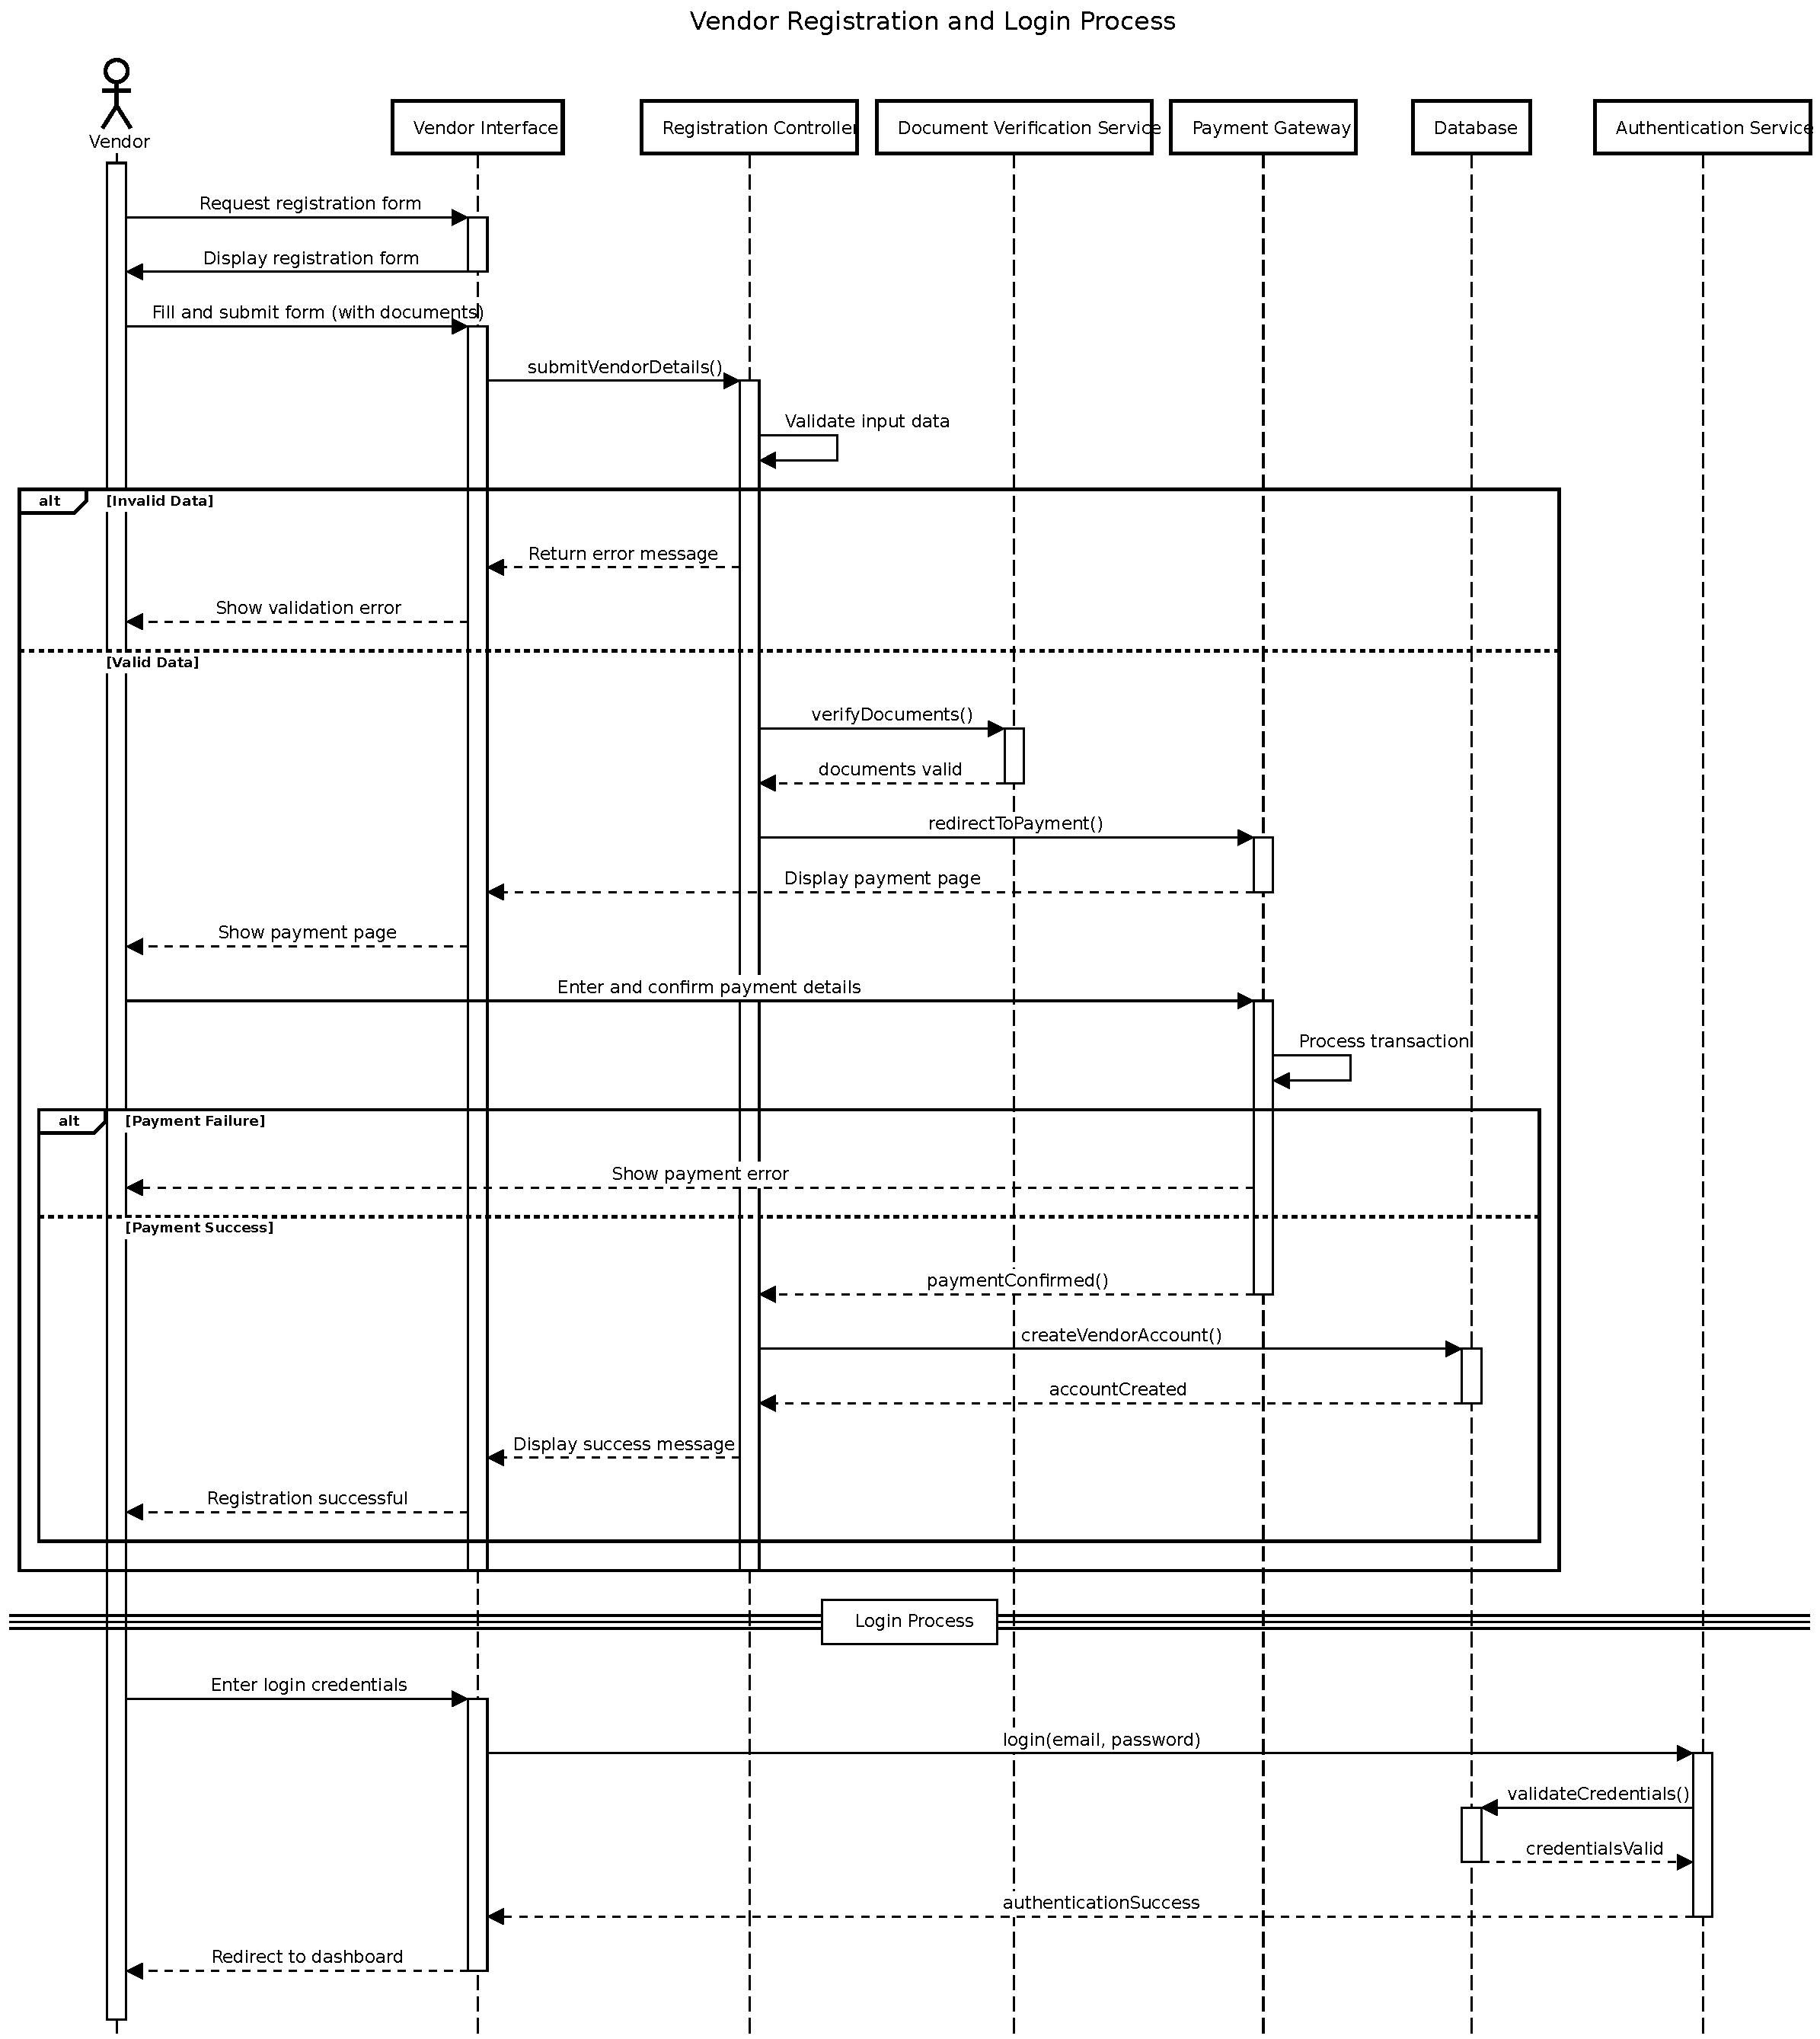
\includegraphics[width=\linewidth]{figures/1. Vendor Login.pdf}
    \caption{Registration & Login Process Diagram}
    \label{fig:delivery_tracking}
\end{figure}


\subsection{Discount and Offer Management Sequence}

\begin{figure}[H] 
    \centering
    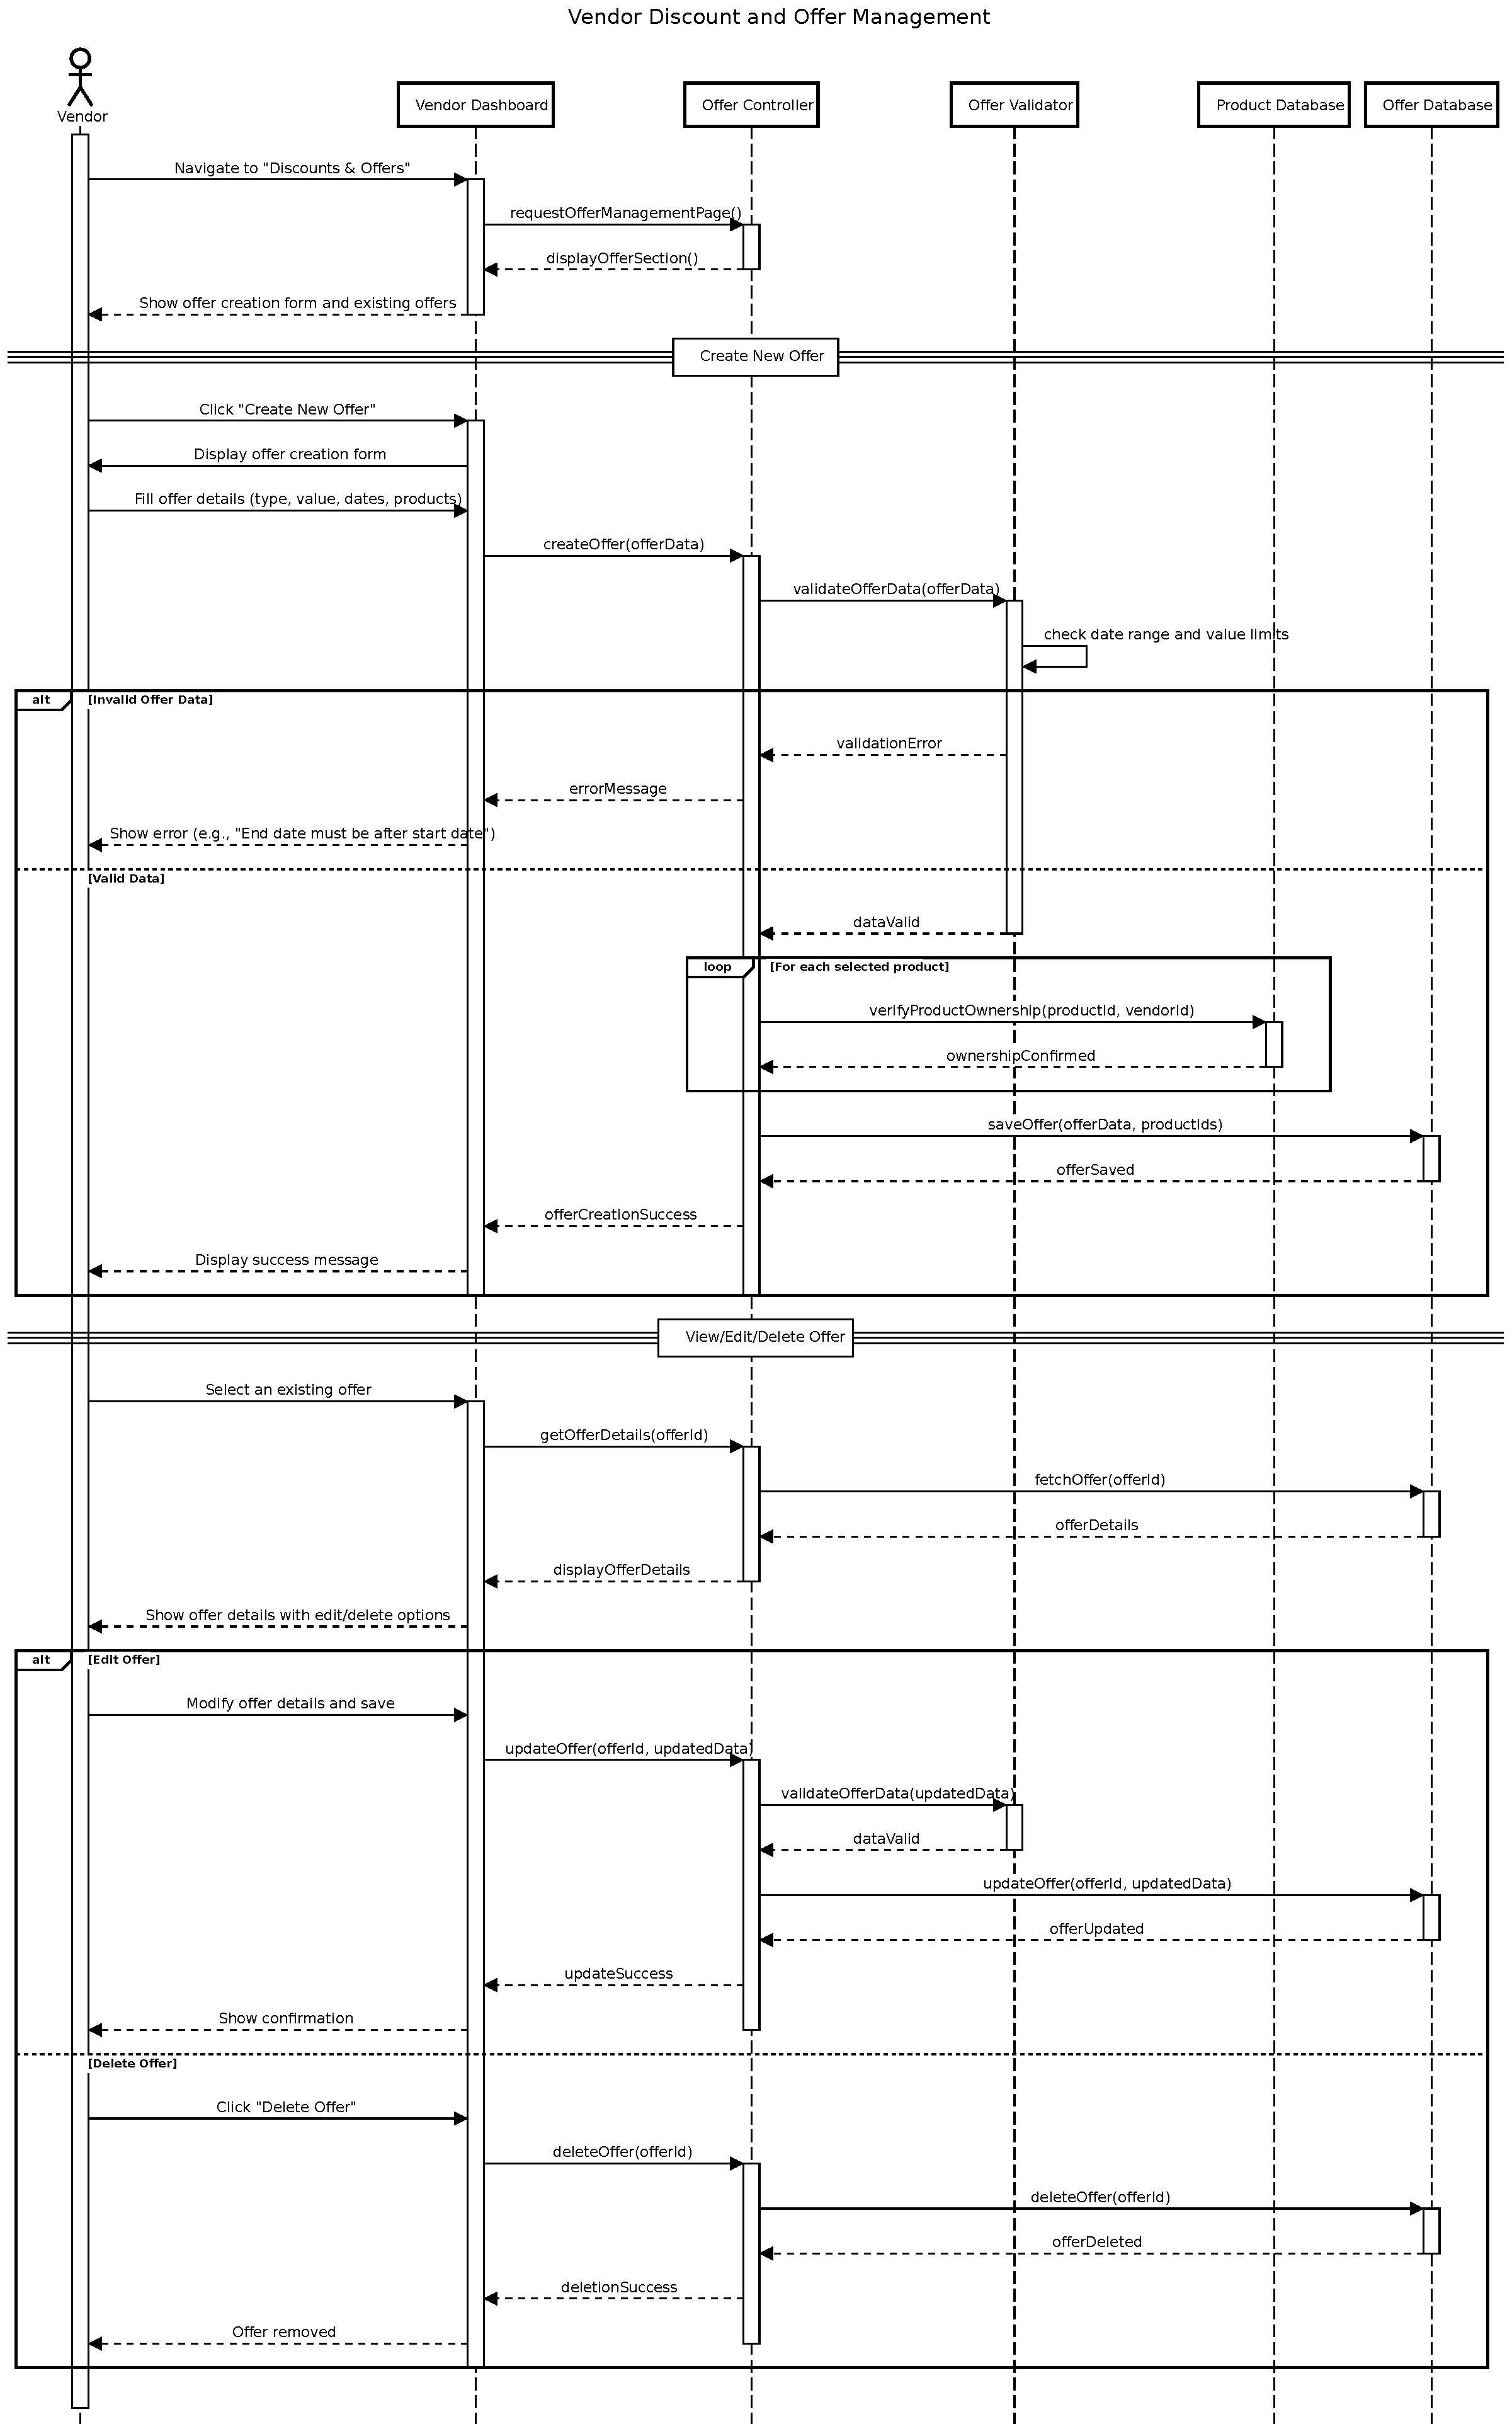
\includegraphics[width=0.8\linewidth]{figures/3. Vendor Discount and offer management.pdf}
    % \includesvg{sqv3}
    \caption{Discount & Offer Management Diagram}
    \label{fig:order_placement}
\end{figure}

\subsection{Vendor Inventory Management Sequence}

\begin{figure}[H]
    \centering
    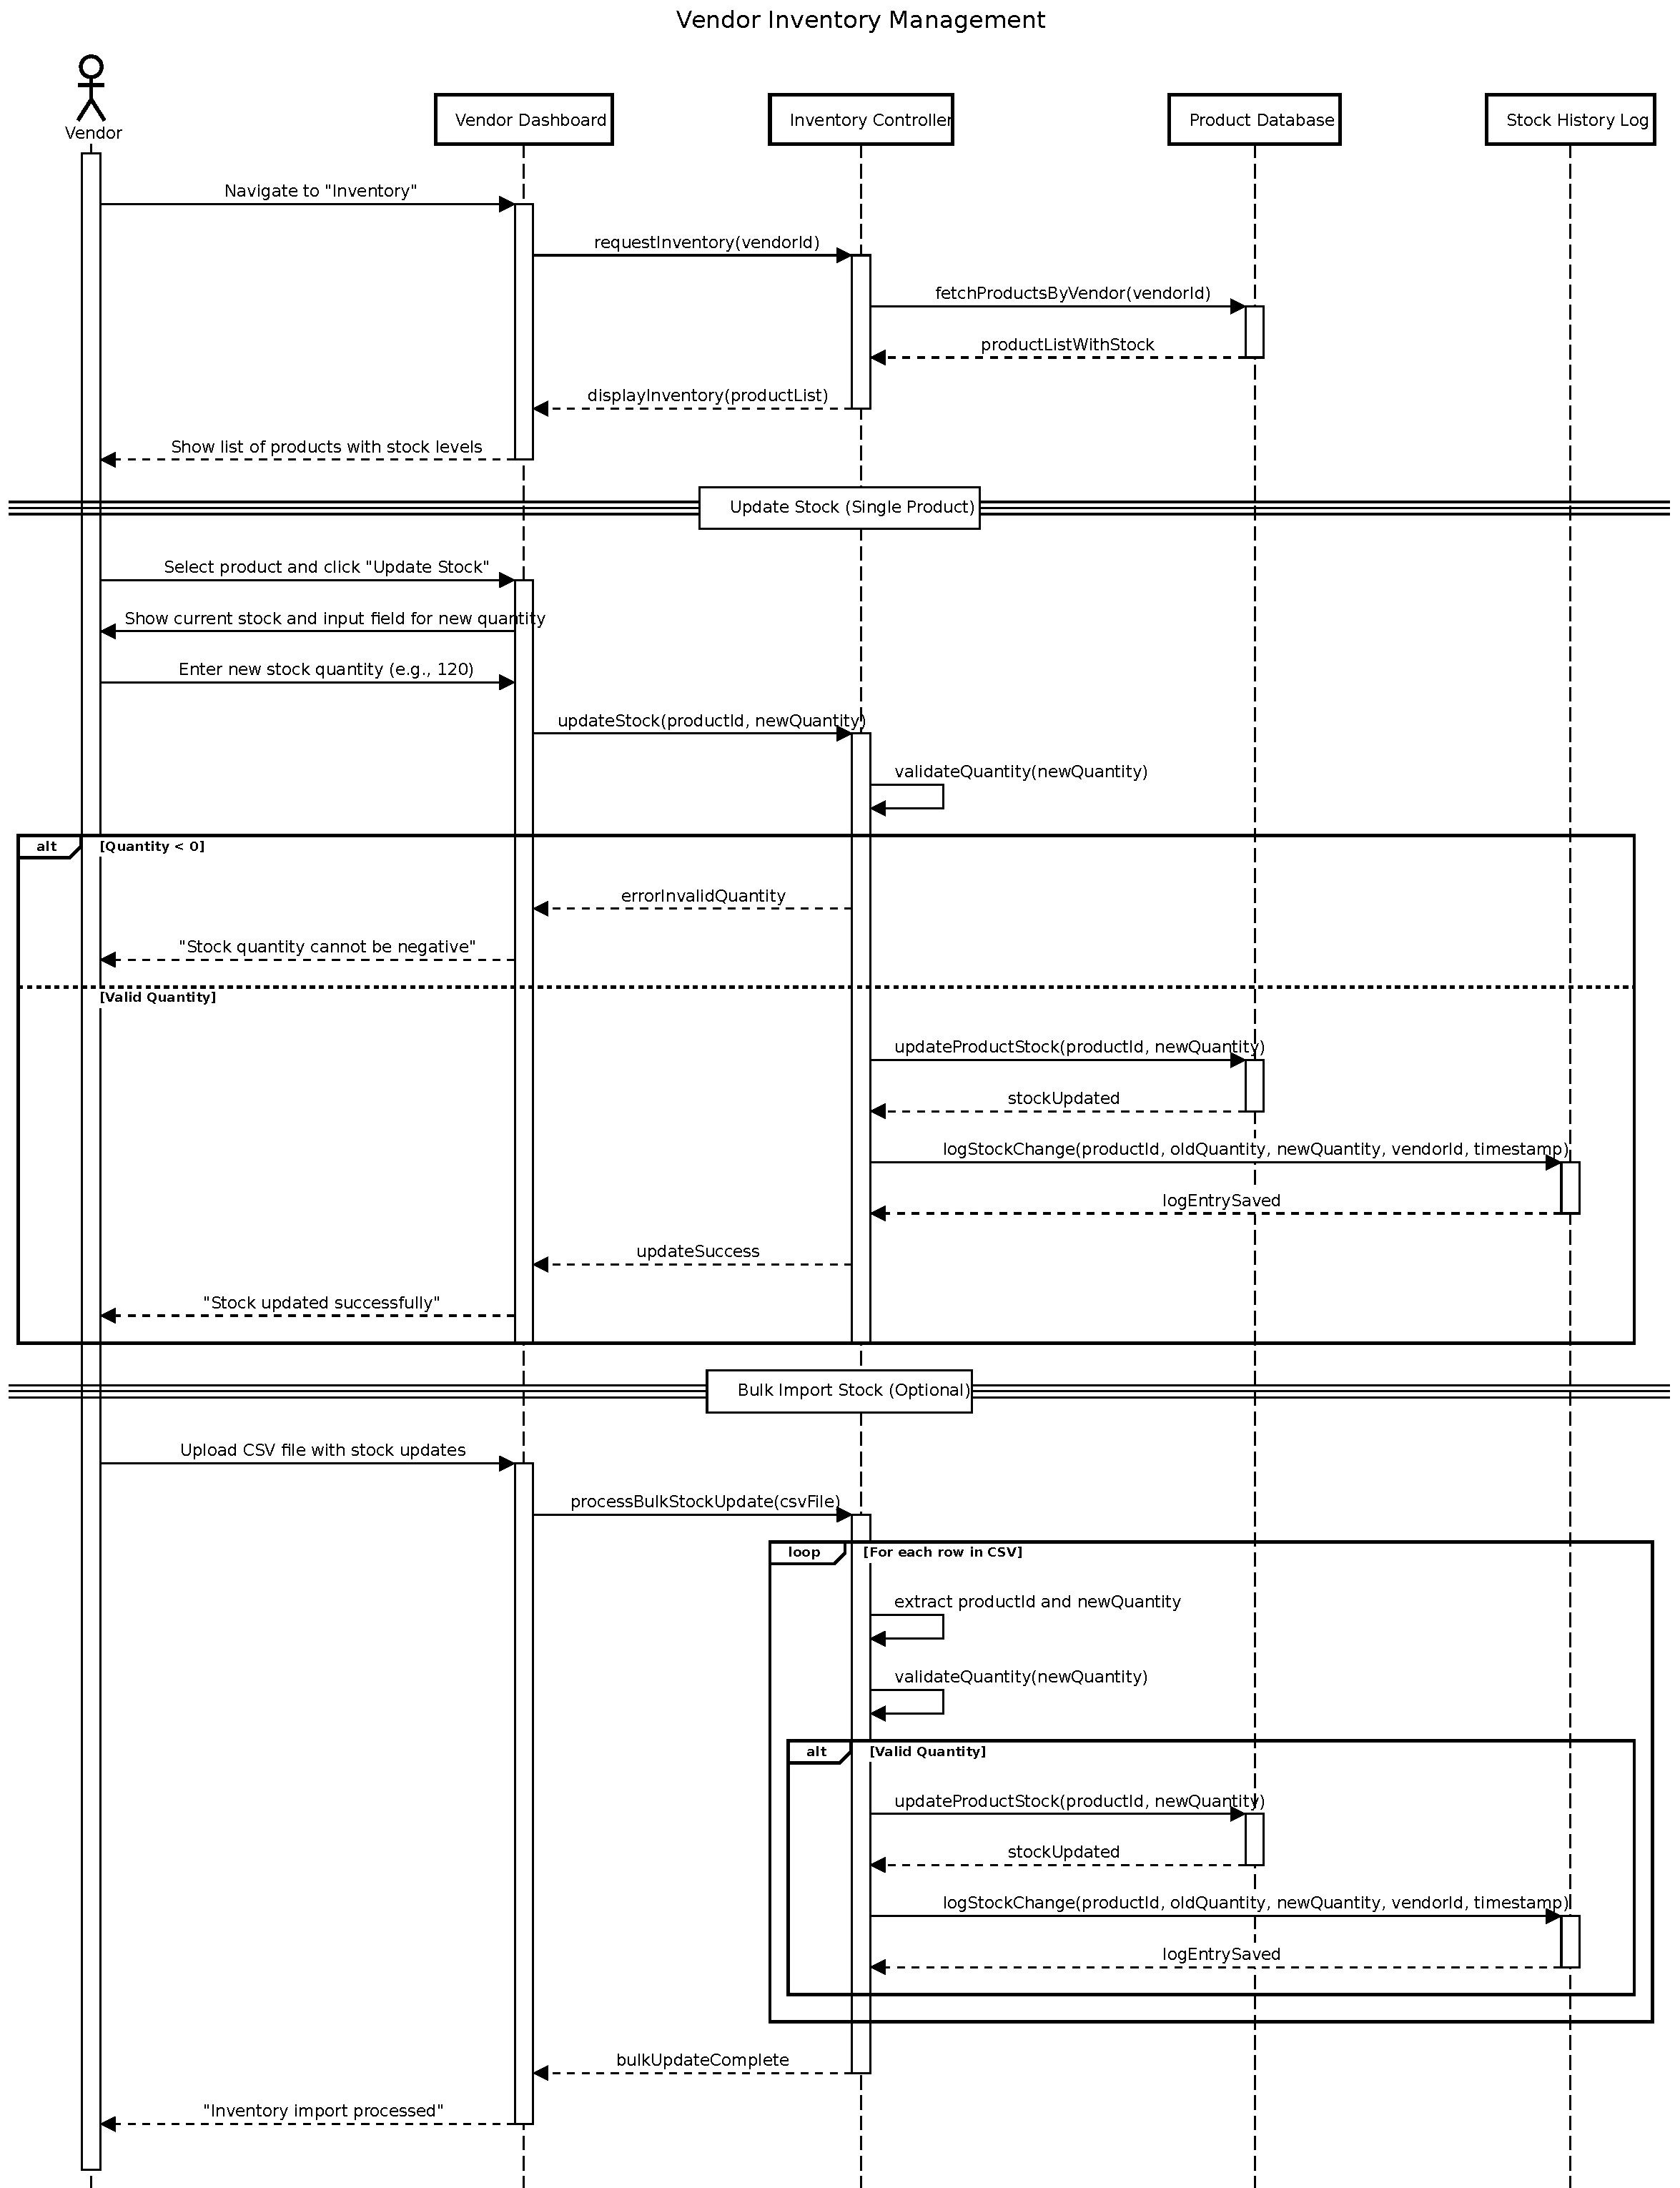
\includegraphics[width=\linewidth]{figures/5. Vendor Inventory.pdf}
    \caption{Vendor Inventory Management Sequence Diagram}
    \label{fig:vendor_registration}
\end{figure}

\subsection{Product Order to Delivery Process Sequence}

\begin{figure}[H]
    \centering
   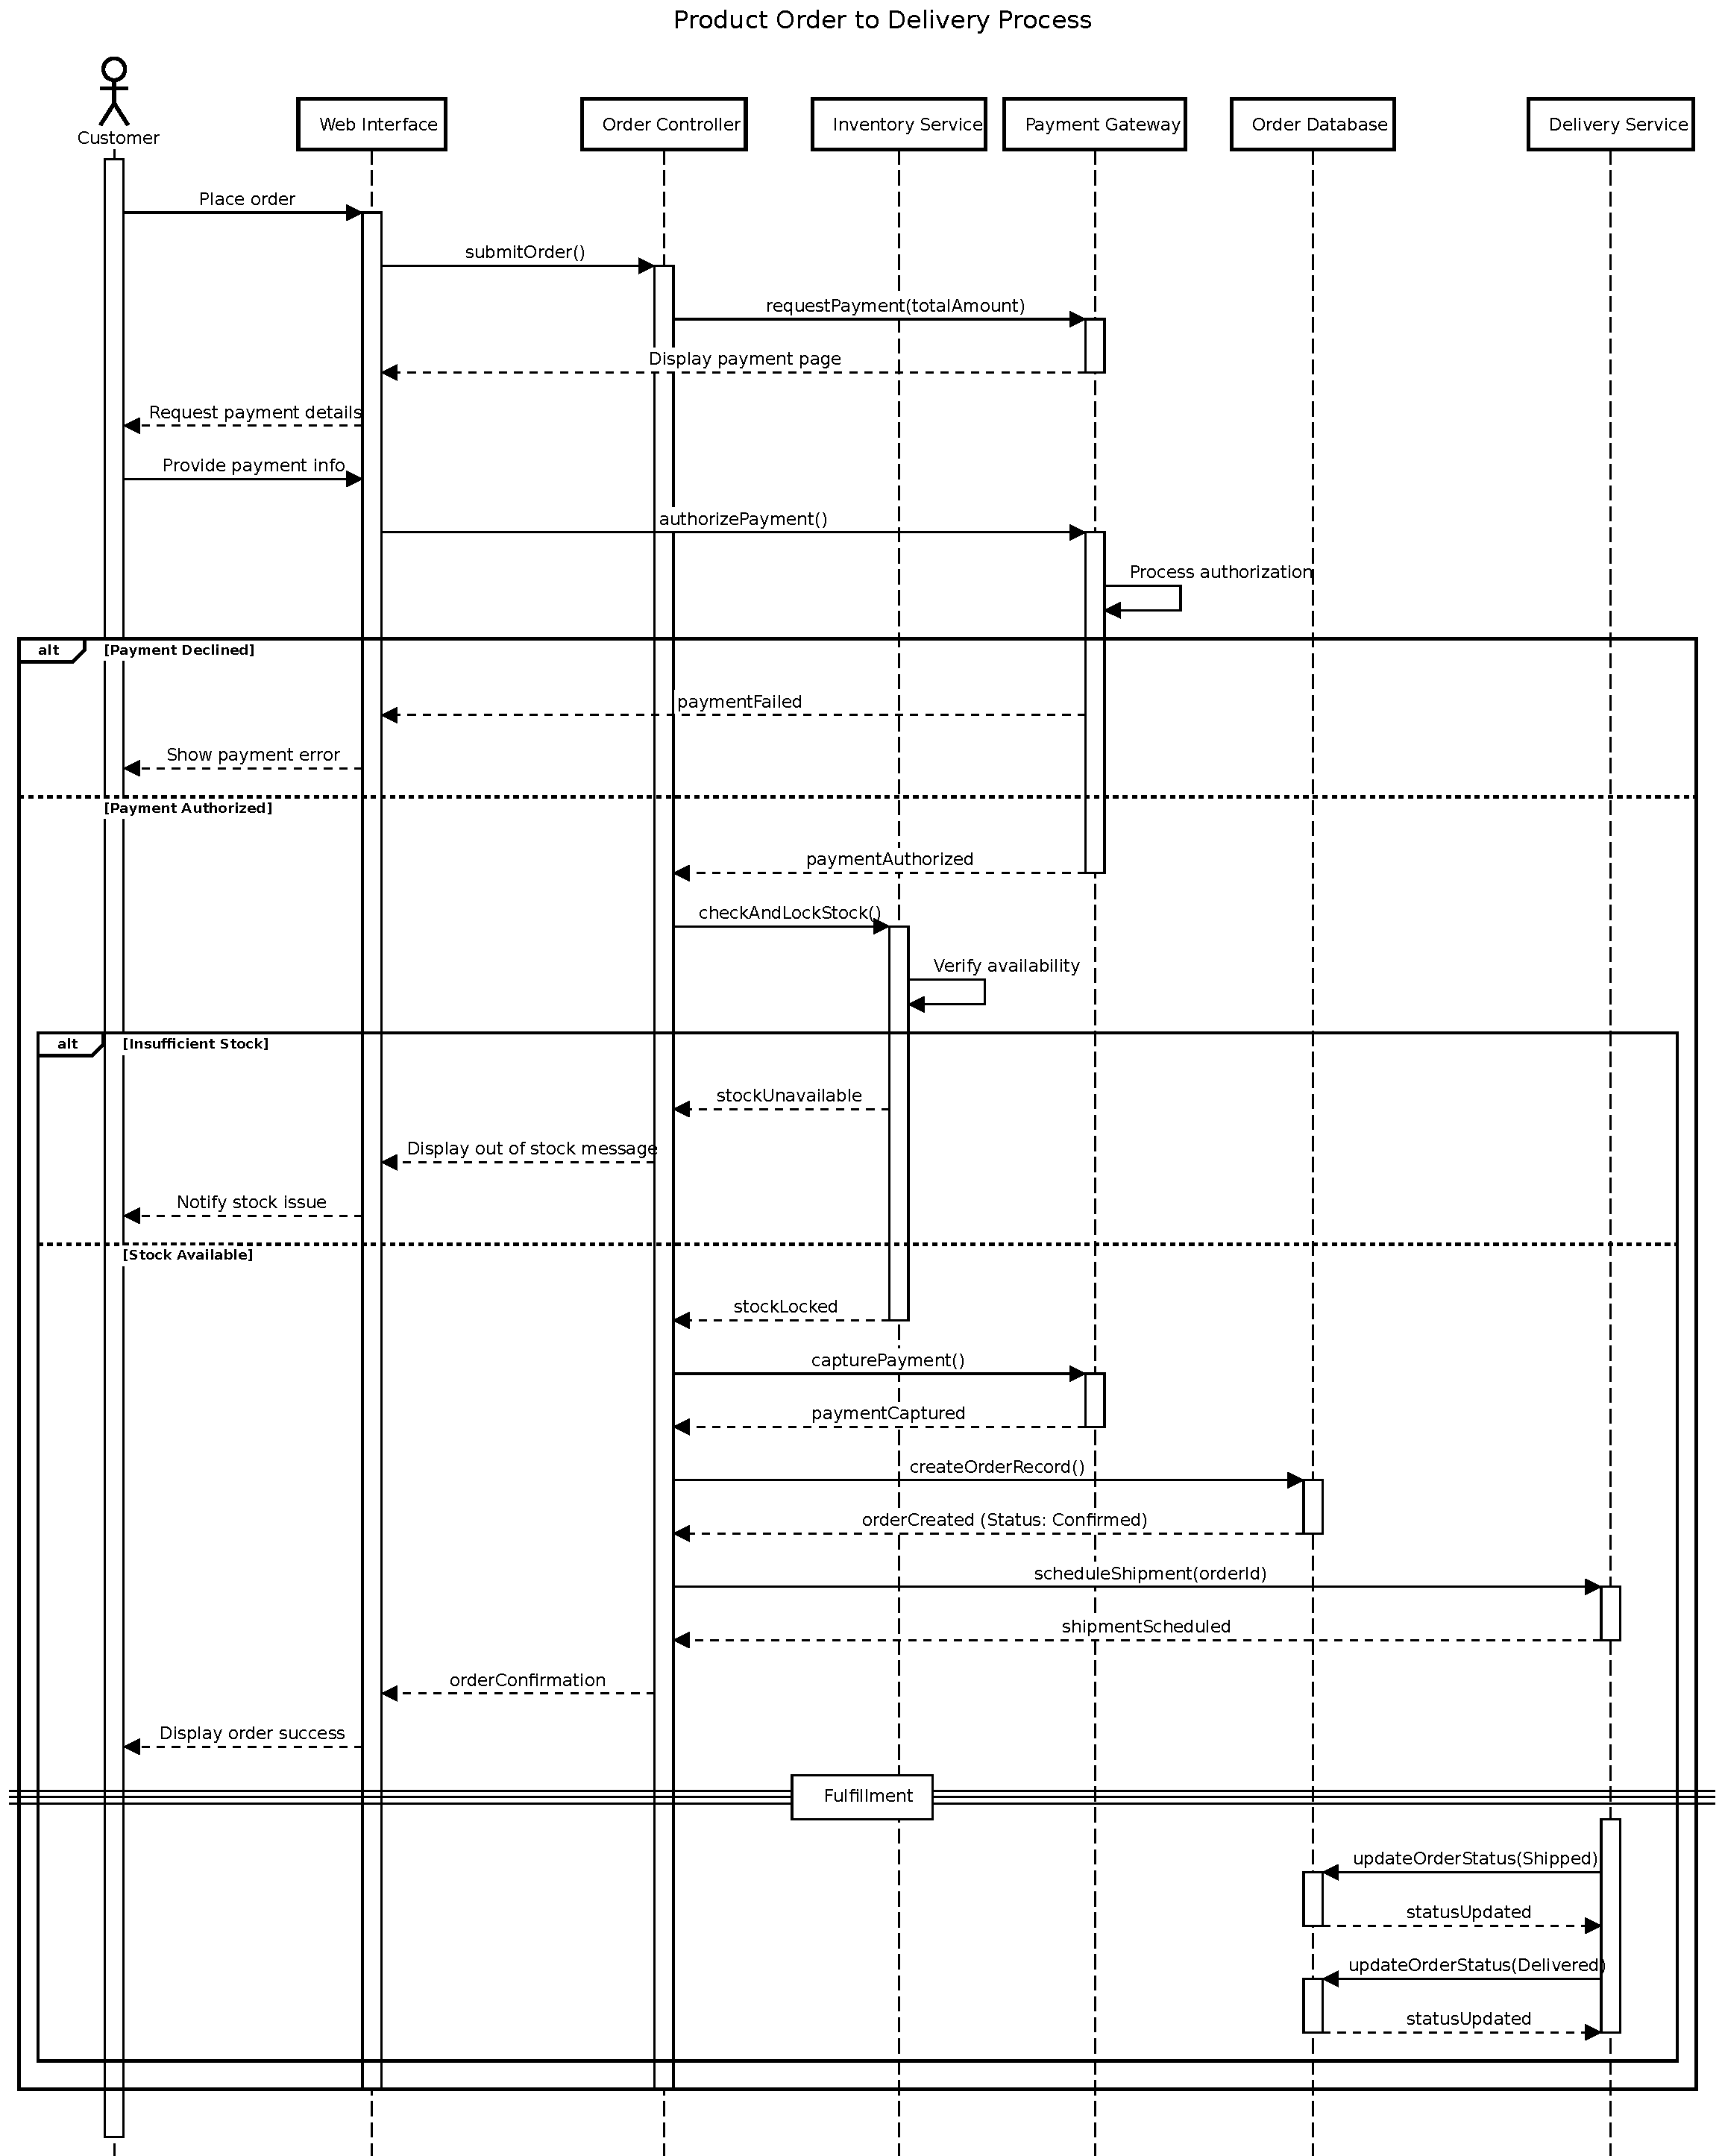
\includegraphics[width=\linewidth]{figures/2. Product order and delicvary.pdf}
    \caption{Payment Processing Sequence Diagram}
    \label{fig:Product Order to Delivery Process diagram}
\end{figure}

\subsection{Rating,Review,Feedback Sequence}

\begin{figure}[H]
    \centering
    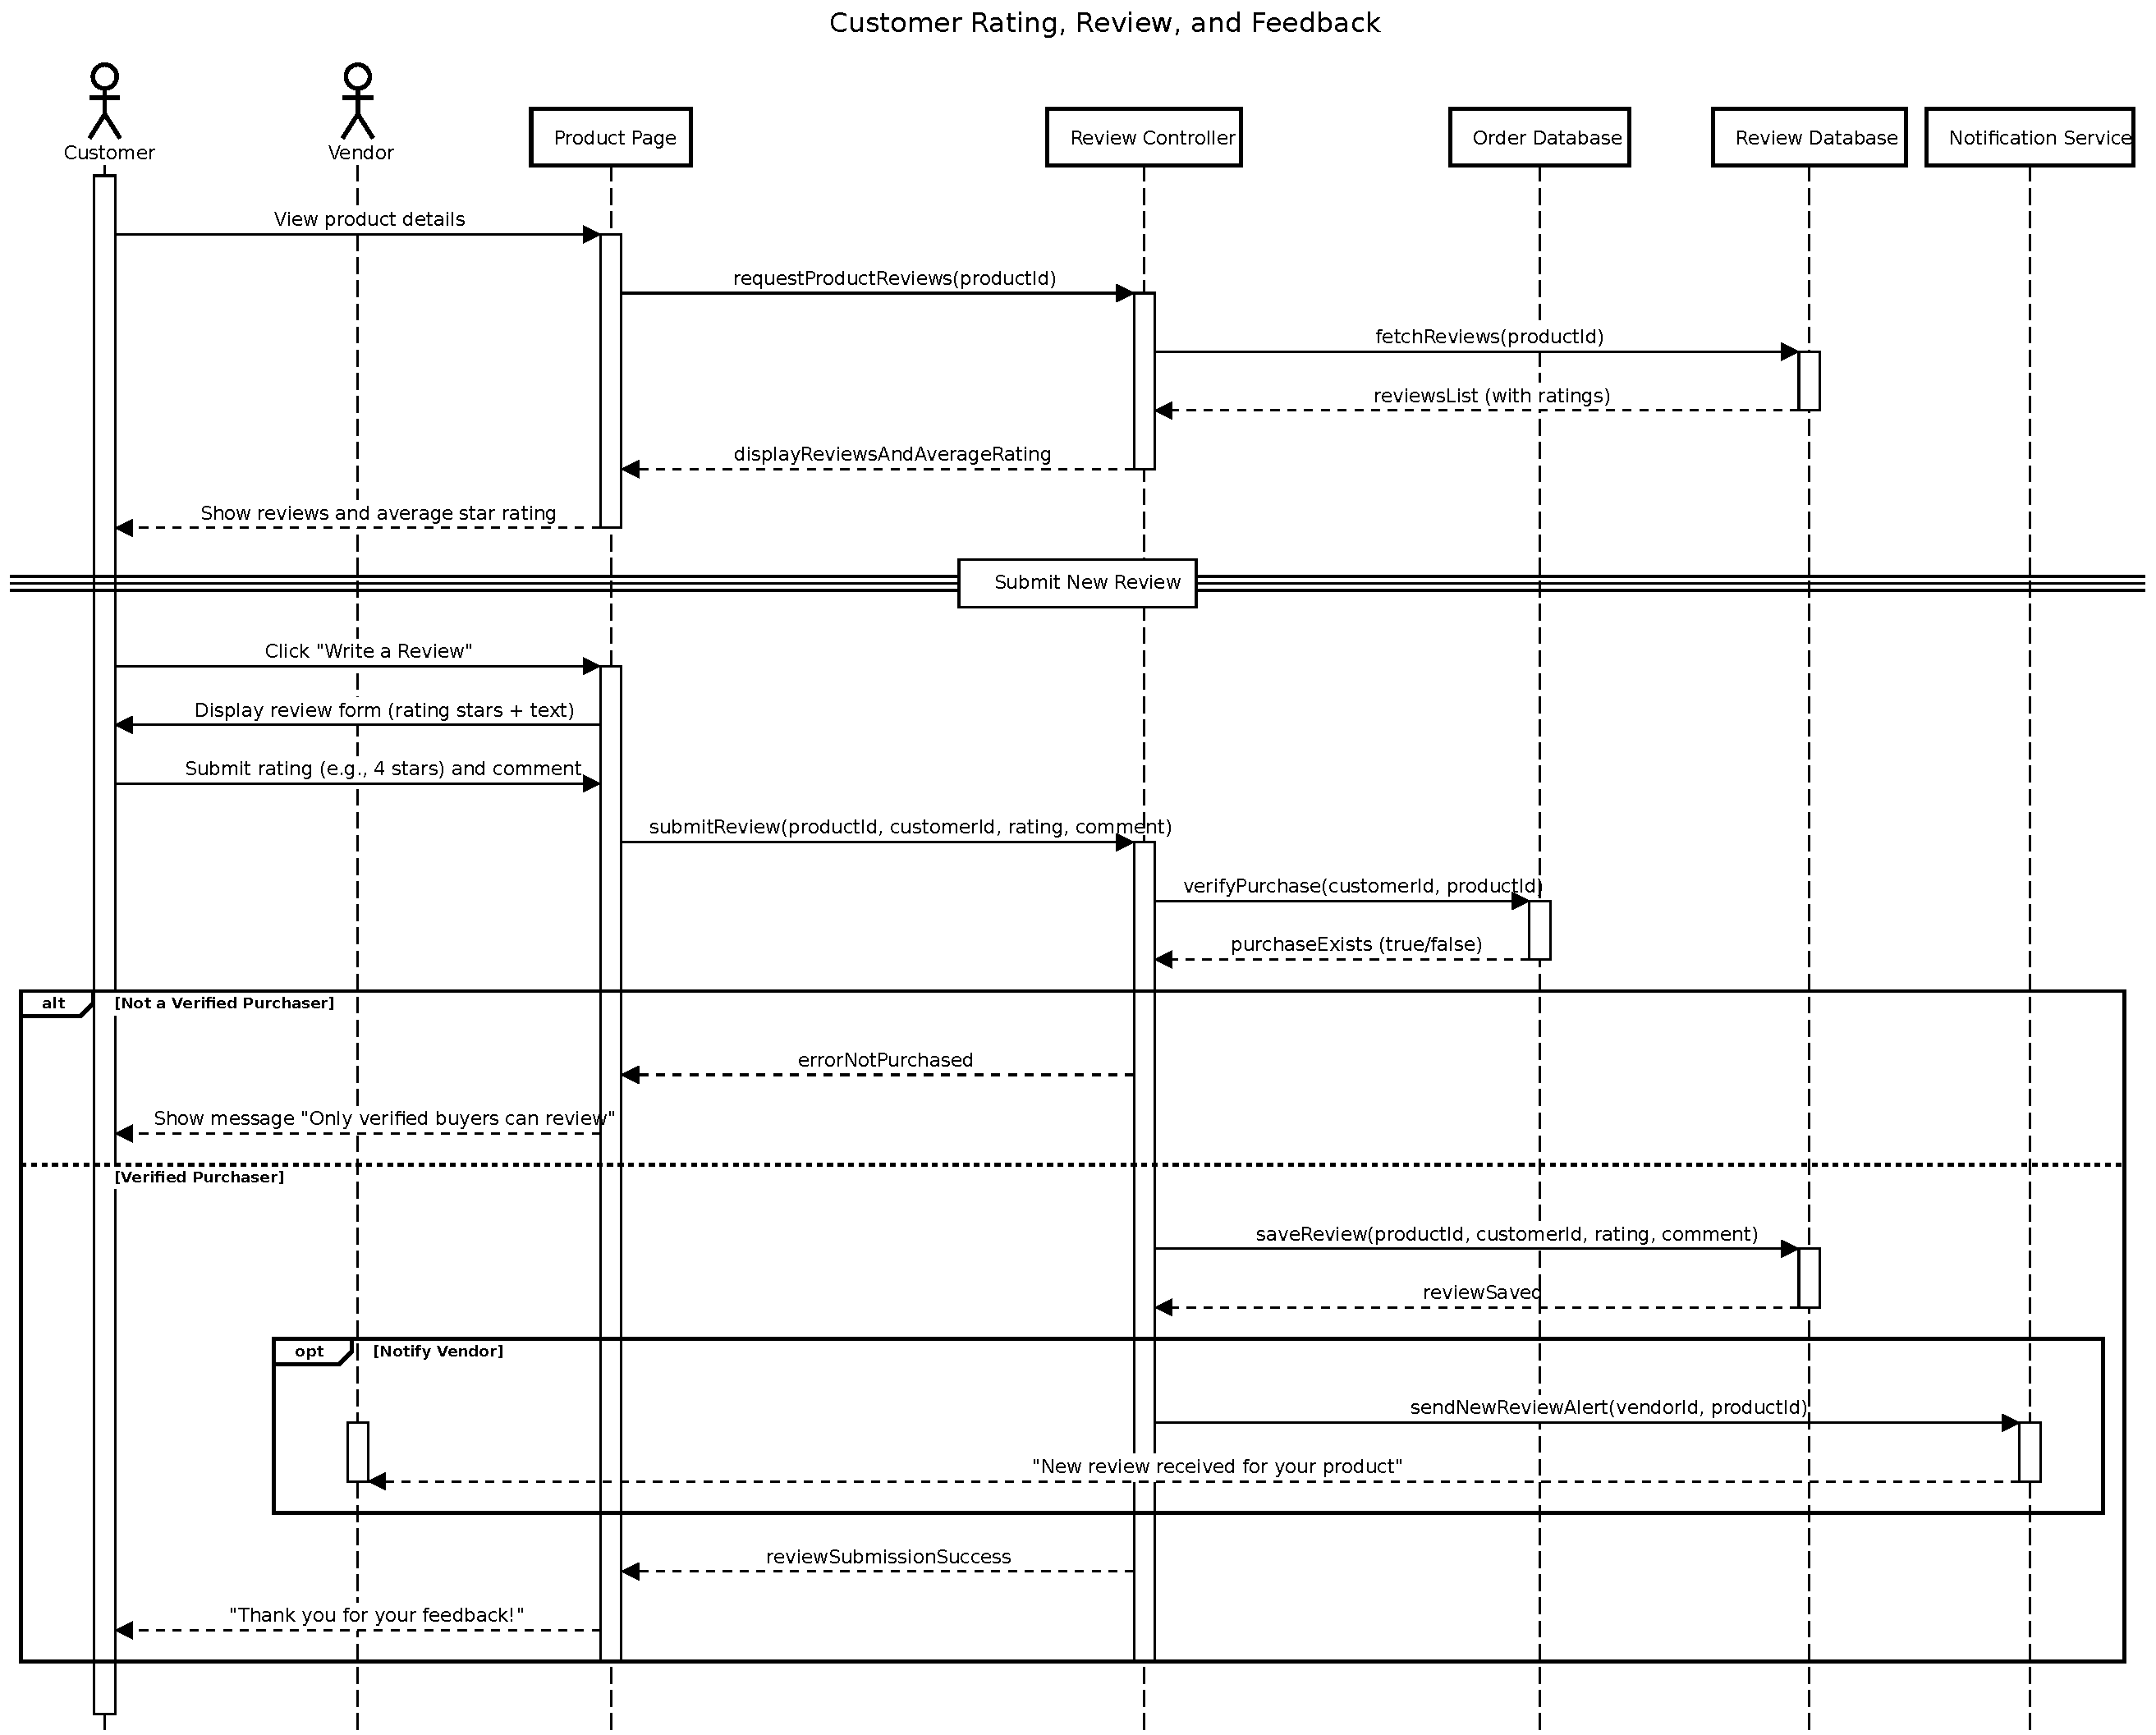
\includegraphics[width=\linewidth]{figures/4. Customer Rating and feedback.pdf}
    \caption{Rating,Review,Feedback Sequence Diagram}
    \label{fig:product_management}
\end{figure}

\section{State Chart Diagram}

\subsection{Registration}

\begin{figure}[H]
    \centering
    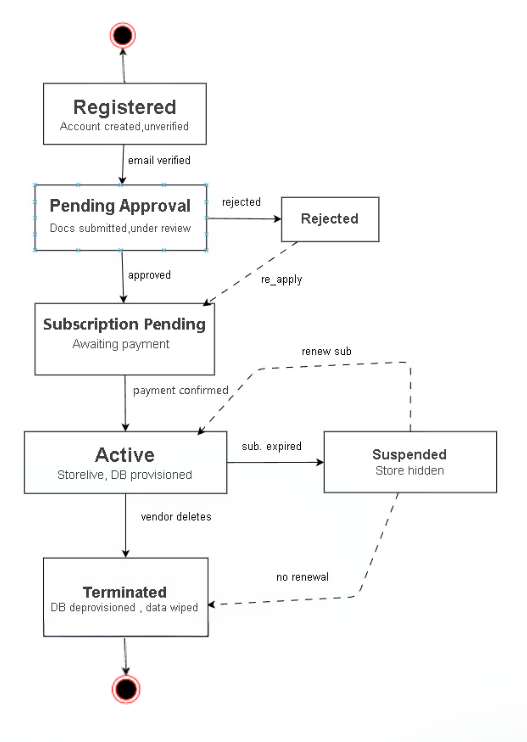
\includegraphics[width=0.8\linewidth]{figures/state chart/vendor.png}
    \caption{Registration State Chart Diagram}
    \label{fig:state_order}
\end{figure}

\subsection{Order Process}

\begin{figure}[H]
    \centering
    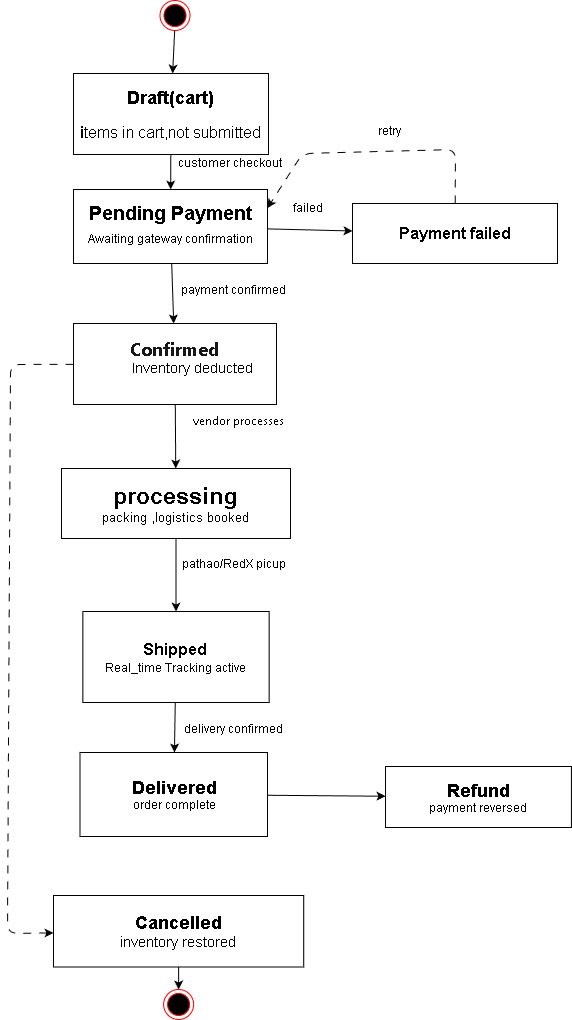
\includegraphics[width=0.8\linewidth]{figures/state chart/order.png}
    \caption{Order Process State Chart Diagram}
    \label{fig:state_vendor}
\end{figure}

\subsection{Payment}

\begin{figure}[H]
    \centering
    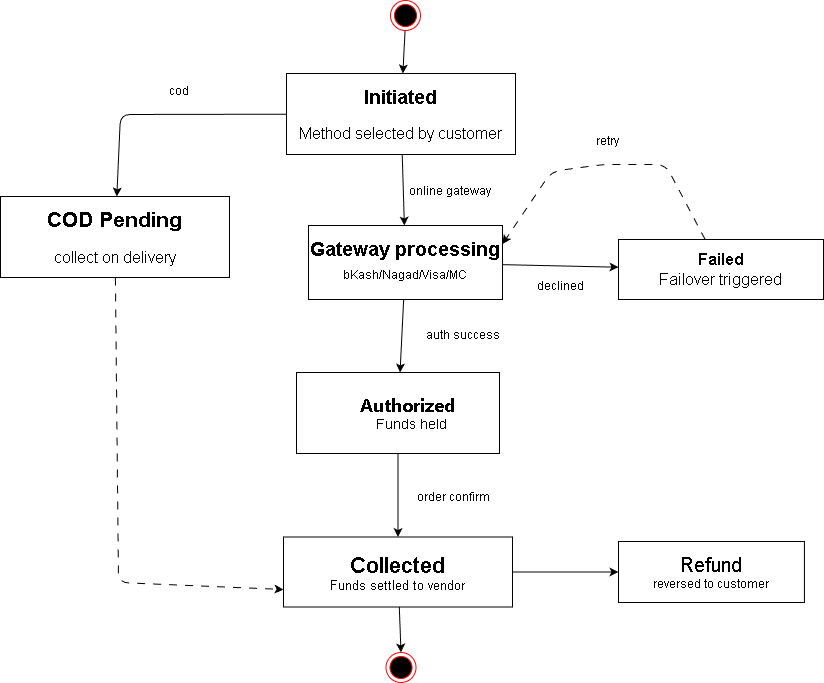
\includegraphics[width=0.8\linewidth]{figures/state chart/payment.png}
    \caption{payment State Chart Diagram}
    \label{fig:state_product}
\end{figure}

\subsection{Delivery}

\begin{figure}[H]
    \centering
    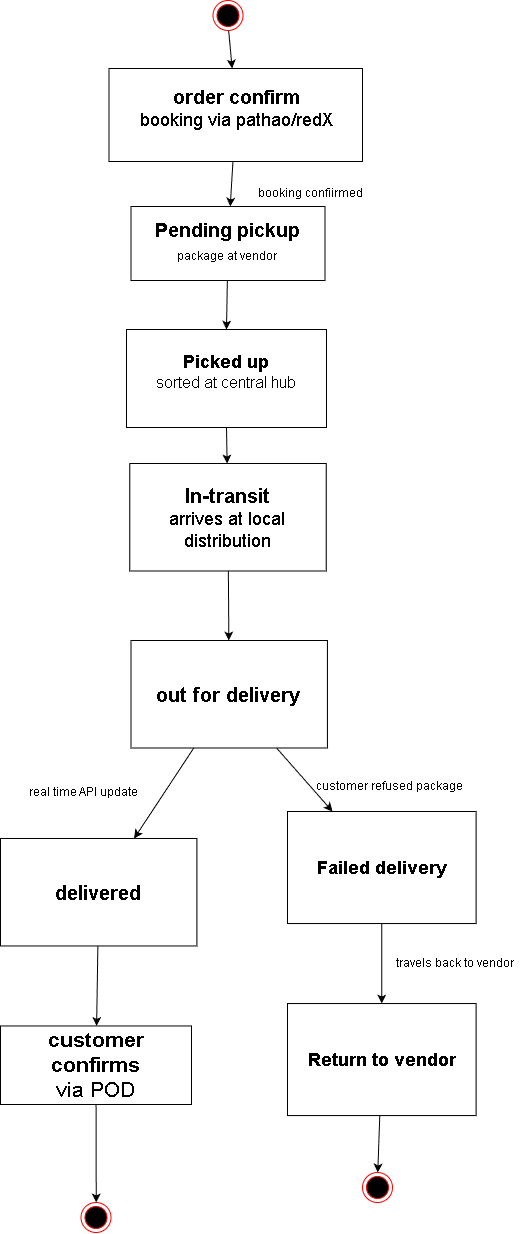
\includegraphics[width=0.6\linewidth]{figures/state chart/delivery.png}
    \caption{delivery State Chart Diagram}
    \label{fig:state_payment}
\end{figure}

\subsection{Inventory}

\begin{figure}[H]
    \centering
    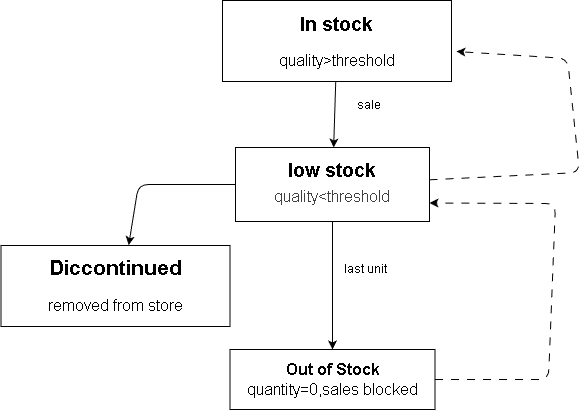
\includegraphics[width=0.8\linewidth]{figures/state chart/inventory.png}
    \caption{Inventory State Chart Diagram}
    \label{fig:state_delivery}
\end{figure}

\section{Database Schema}

\begin{figure}[H]
    \centering
    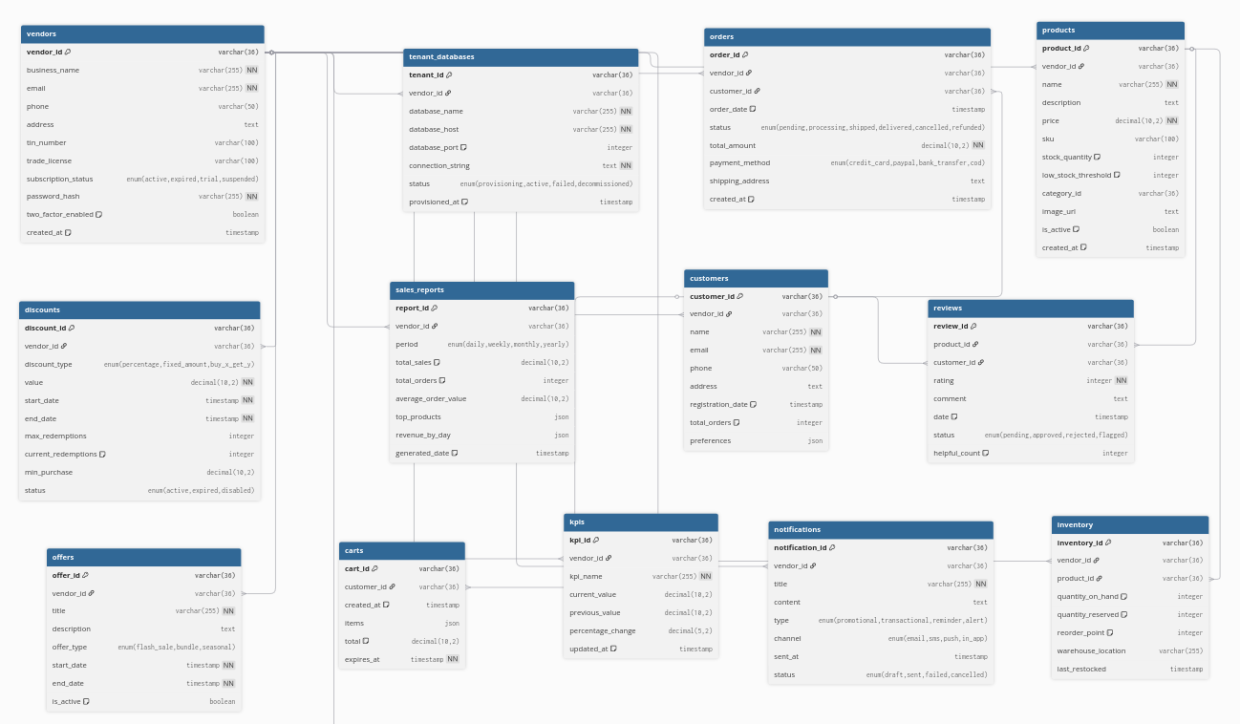
\includegraphics[width=1\linewidth]{figures/schema.png}
    \caption{Database Schema for Multi-Tenants E-Commerce System}
    \label{fig:placeholder}
\end{figure}